\section{Seguimiento longitudinal}
Este capitulo contiene cuatro secciones las cuales abordan respectivamente la evolución de los \textbf{cotizantes dependientes del sector privado}\footnote{Se excluye del análisis los dependientes del sector NO-Privado} e \textbf{independientes} respecto de sus dinámica de salidas, entradas y distribución demográfica de los cotizantes al SPS. En este capitulo se habla de entradas, permanencias y salidas, para ver su definición refiérase al Anexo \ref{fig:anexo:glosario}.

\subsection{Resumen de entradas y salidas del SPS}
La figura \ref{figura:dependientes:entradas_salidas} muestra la evolución de las \textcolor{green}{entradas} y \textcolor{red}{salidas} de cotizantes al SPS. El comparativo anual se realiza de manera mensual a lo largo del último semestre. Se puede observar que el número de nuevos cotizantes disminuye para el mes de Diciembre, comportamiento que coincide con el aumento en el número de salidas. El comportamiento de las entradas y salidas para los dependientes es atípica para el año 2020 donde los porcentajes están por debajo de lo sucedido para los años 2019 y 2021. Esta diferencia puede explicarse por el impacto rezagado de la pandemia por COVID-19 que tuvo un mayor impacto en la dinámica general de las cotizaciones durante el primer semestre de 2020. En cuanto a los independientes, el comportamiento de las entradas al SPS muestra que el 2021 cierra el año con un porcentaje mayor de entradas, y consecuentemente un porcentaje de salidas mayor durante el último semestre del año. 

\begin{figure}[!htbp]
\centering
\begin{minipage}{0.5\textwidth}
  \centering
  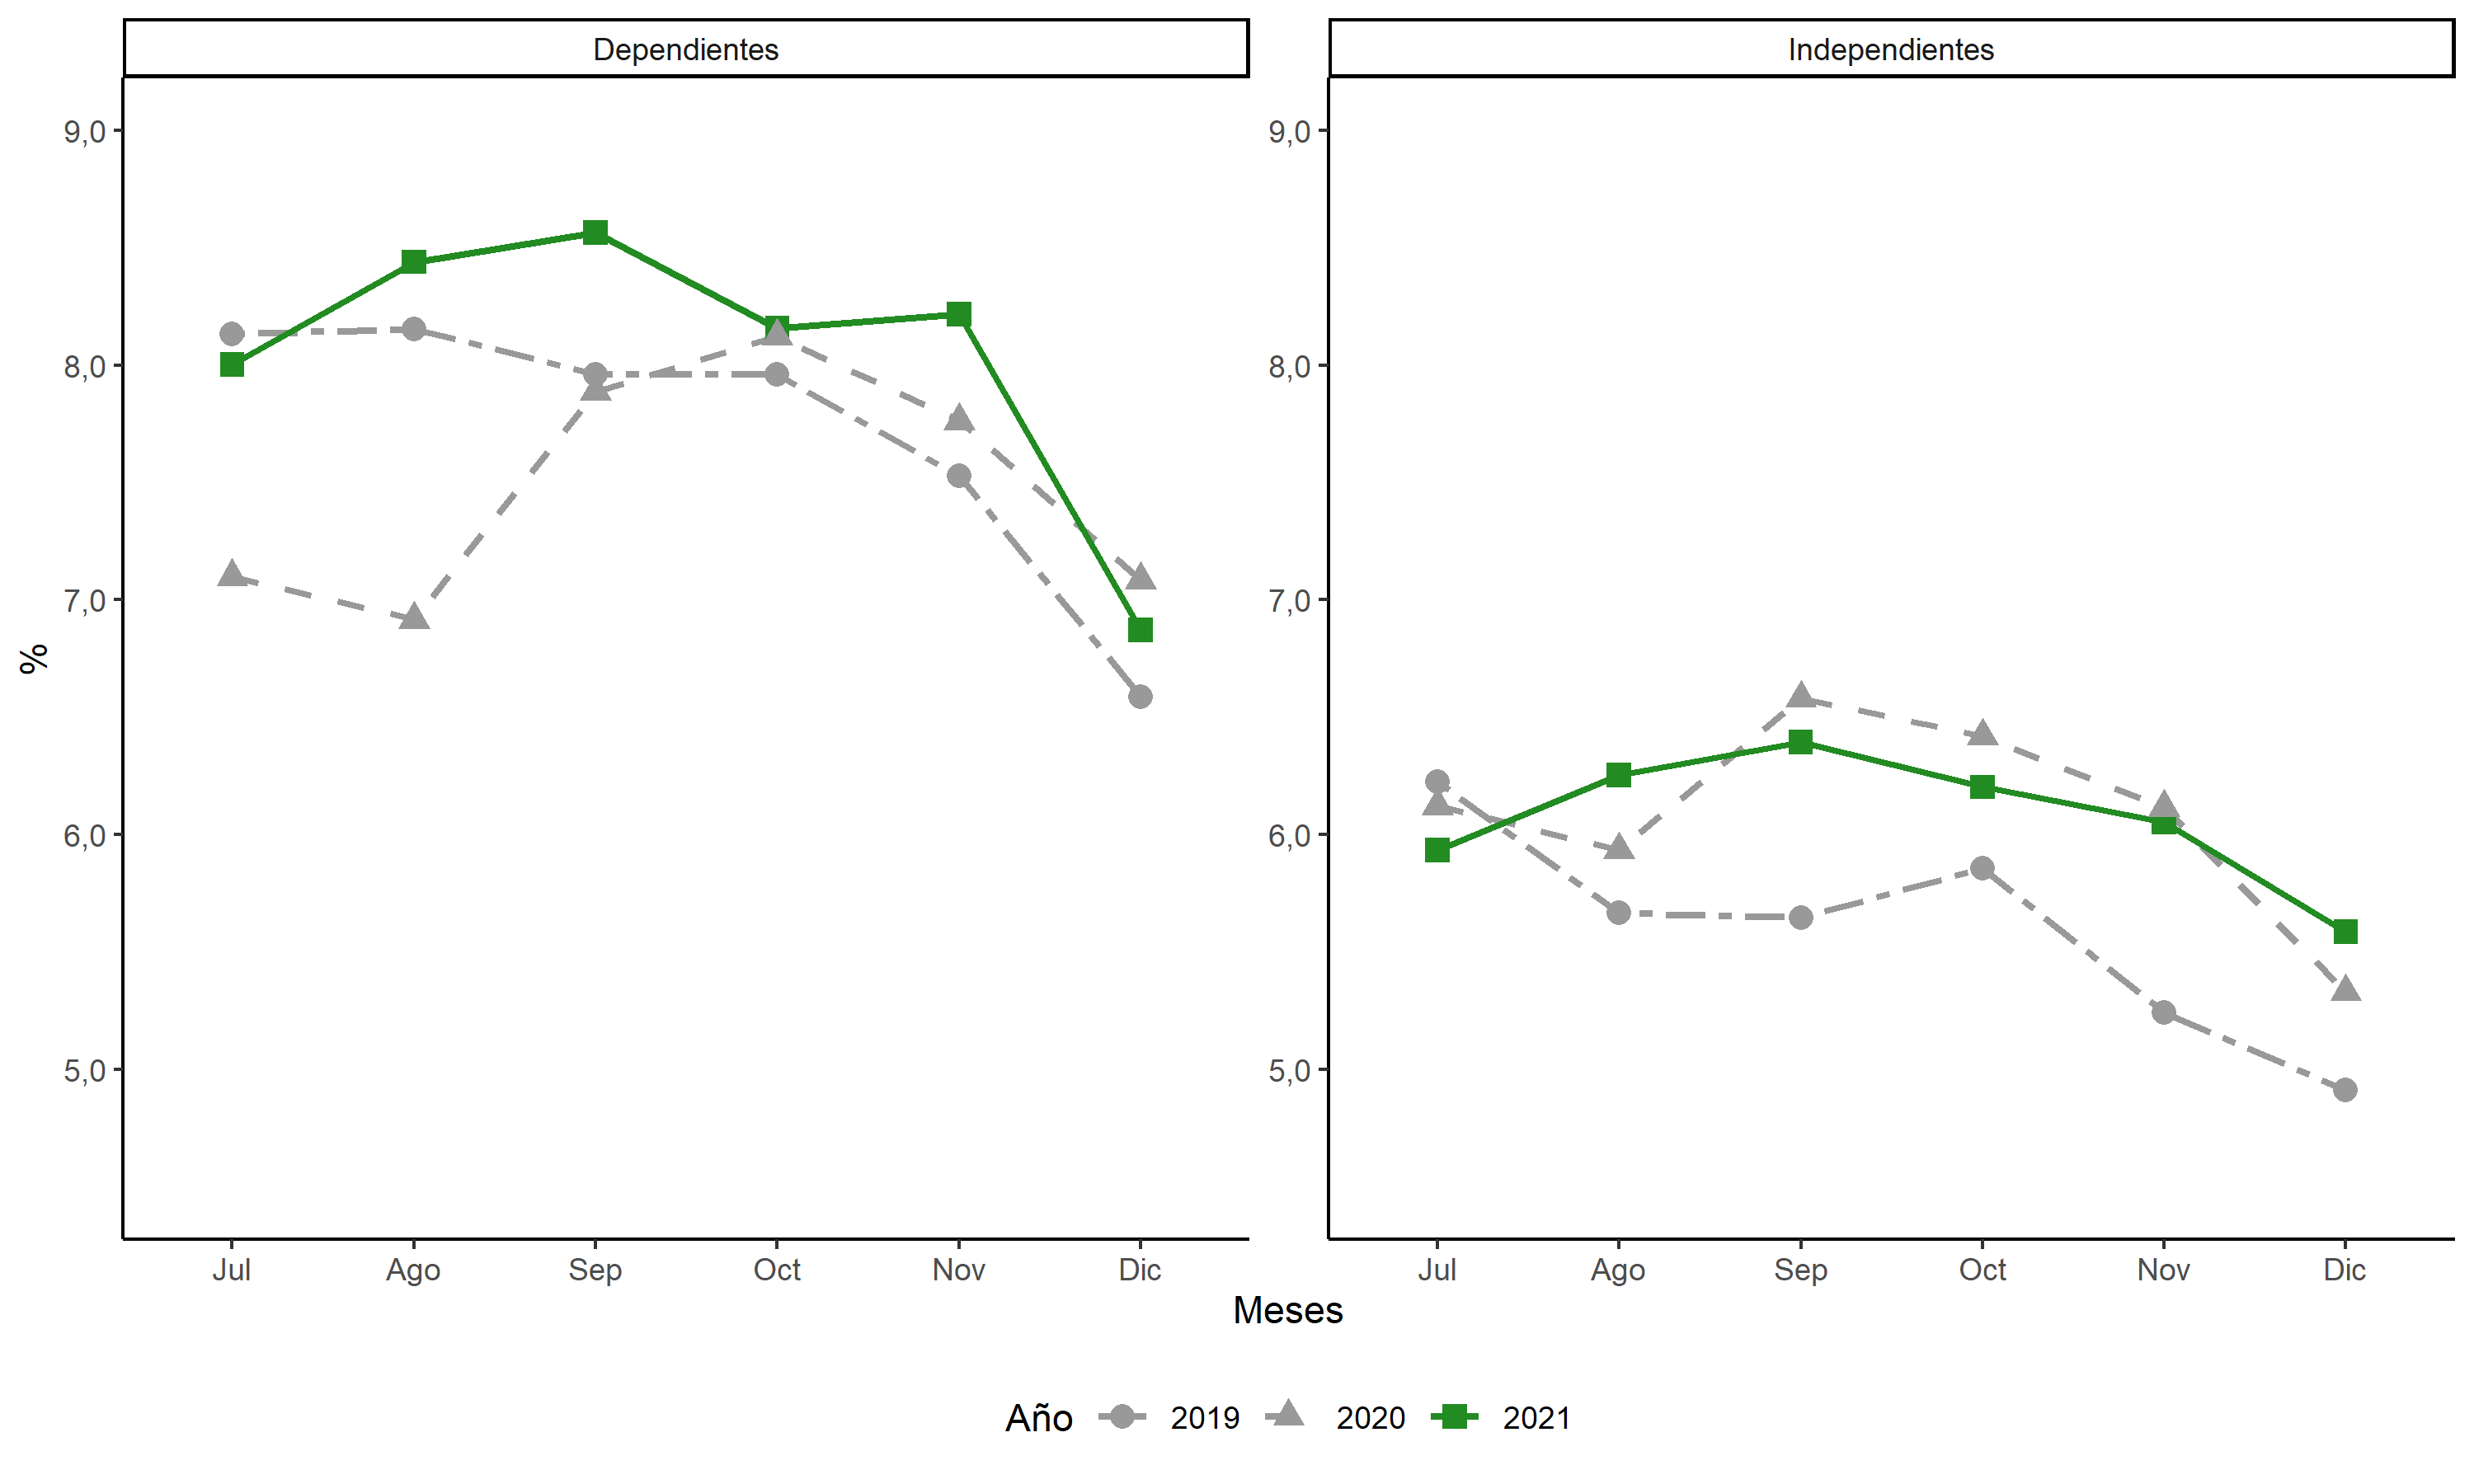
\includegraphics[width=\linewidth]{figures/02_longitudinal/entradas_anual_dependiente_independiente.png}
\end{minipage}%

\begin{minipage}{0.5\textwidth}
  \centering
  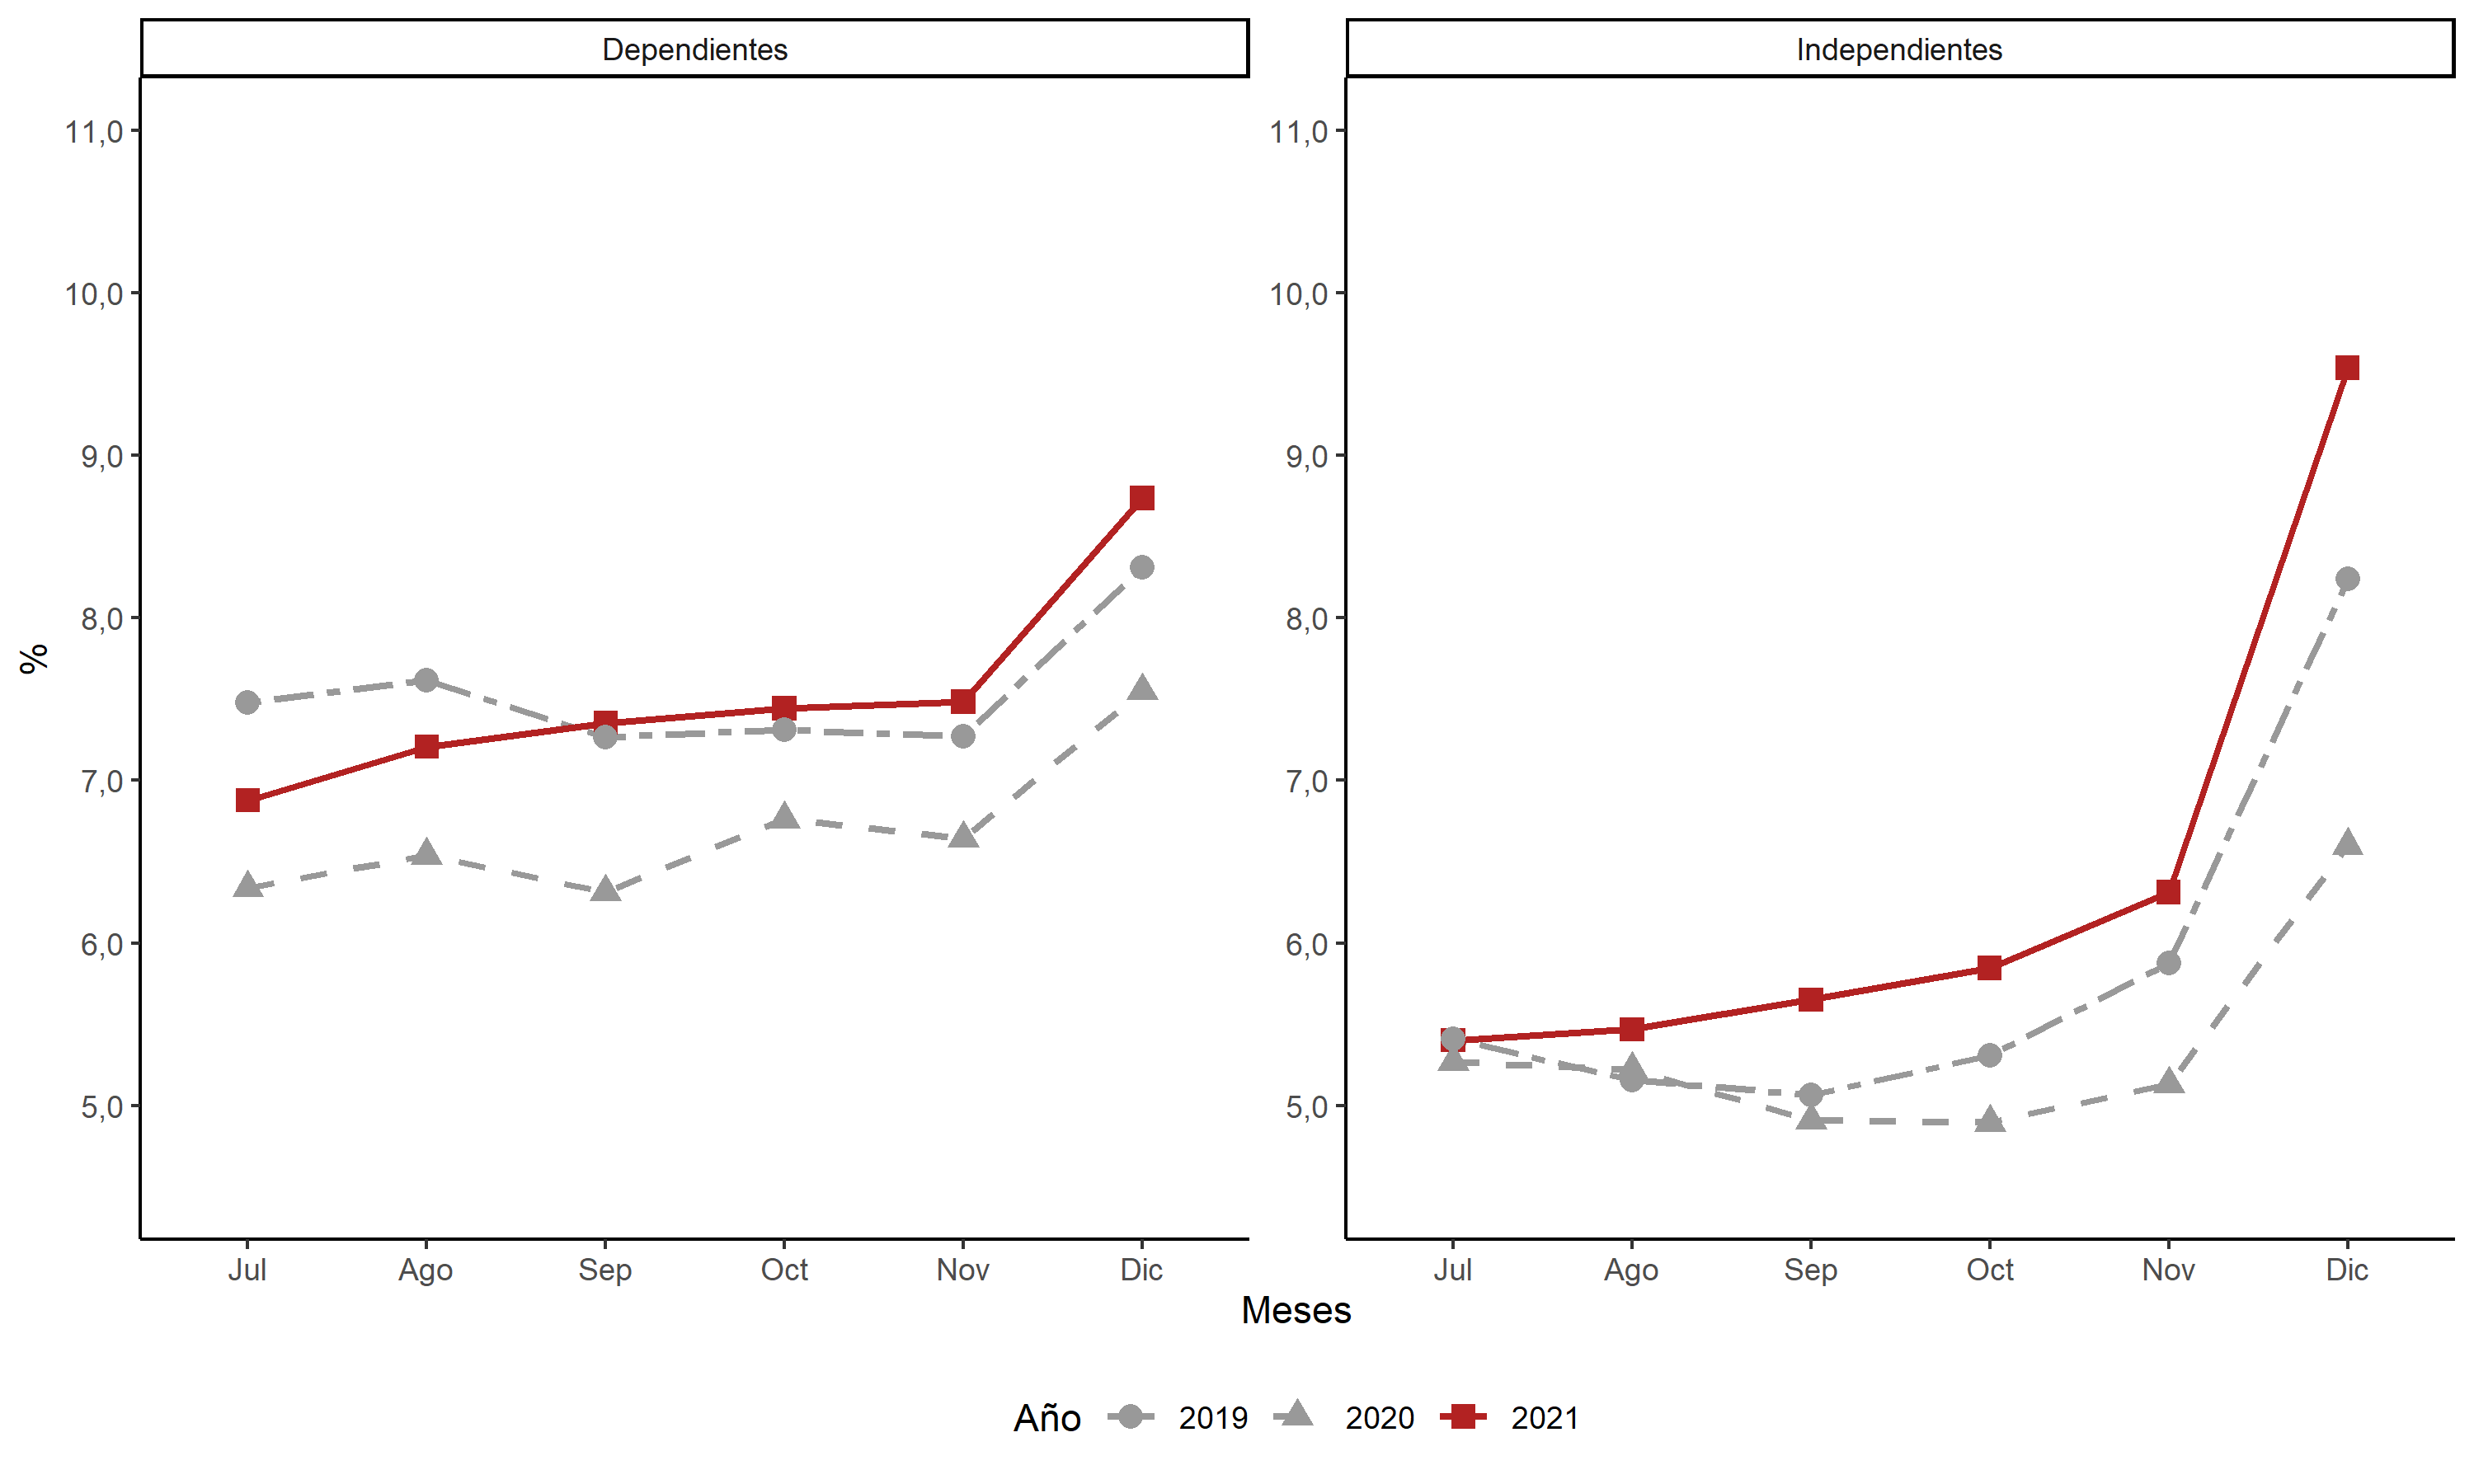
\includegraphics[width=\linewidth]{figures/02_longitudinal/salidas_anual_dependiente_independiente.png}
\end{minipage}
\caption{Porcentaje de entradas (izq.) y salidas (der.) por año)}
\label{figura:dependientes:entradas_salidas}
\end{figure}

\FloatBarrier
\subsection{Cotizantes dependientes del Sector privado}
\subsubsection{Dinámica de entradas y salidas del SPS}
En Diciembre 2021 entraron, permanecieron y salieron 598.204, \textbf{8.106.864} y 776.052 relaciones laborales dependientes del sector privado. Las entradas superan en 22.940 y 46.784 las entradas en 2020 y 2019, las salidas en este periodo también supera a las de 2020 y 2019 en 159.722 y 67.120 relaciones laborales. 

Las entradas en diciembre 2021 corresponden al 6.8\% de las relaciones laborales en este periodo siendo inferior al observado en 2020 y superior al obtenido en 2019 que fueron del 7.08\% y 6.5\%. Las dinámicas en rangos inferiores a los 2 SMMLV o menos son más altos como se muestra en el cuadro \ref{tabla:sector_privado:matriz_dinamica_mes_interes_21} , las entradas de 1 SMMLV o menos son inferiores a los observados en 2020 y superiores a las observadas en 2019, que fueron del 16.3\% y 15.3\%, probablemente sea por el aumento de permanencias que aumentaron en 561.969 y en 288.017 con relación a relaciones laborales de 1 o menos SMMLV en 2020 y 2019 respectivamente. Por otro lado, las salidas son el 8.7\% de relaciones laborales en noviembre 2021, superando al porcentaje de salidas en 2020 y 2019 que fueron de 7.55\% y 8.31\% respectivamente. 

\begin{table}[!htbp]
\centering
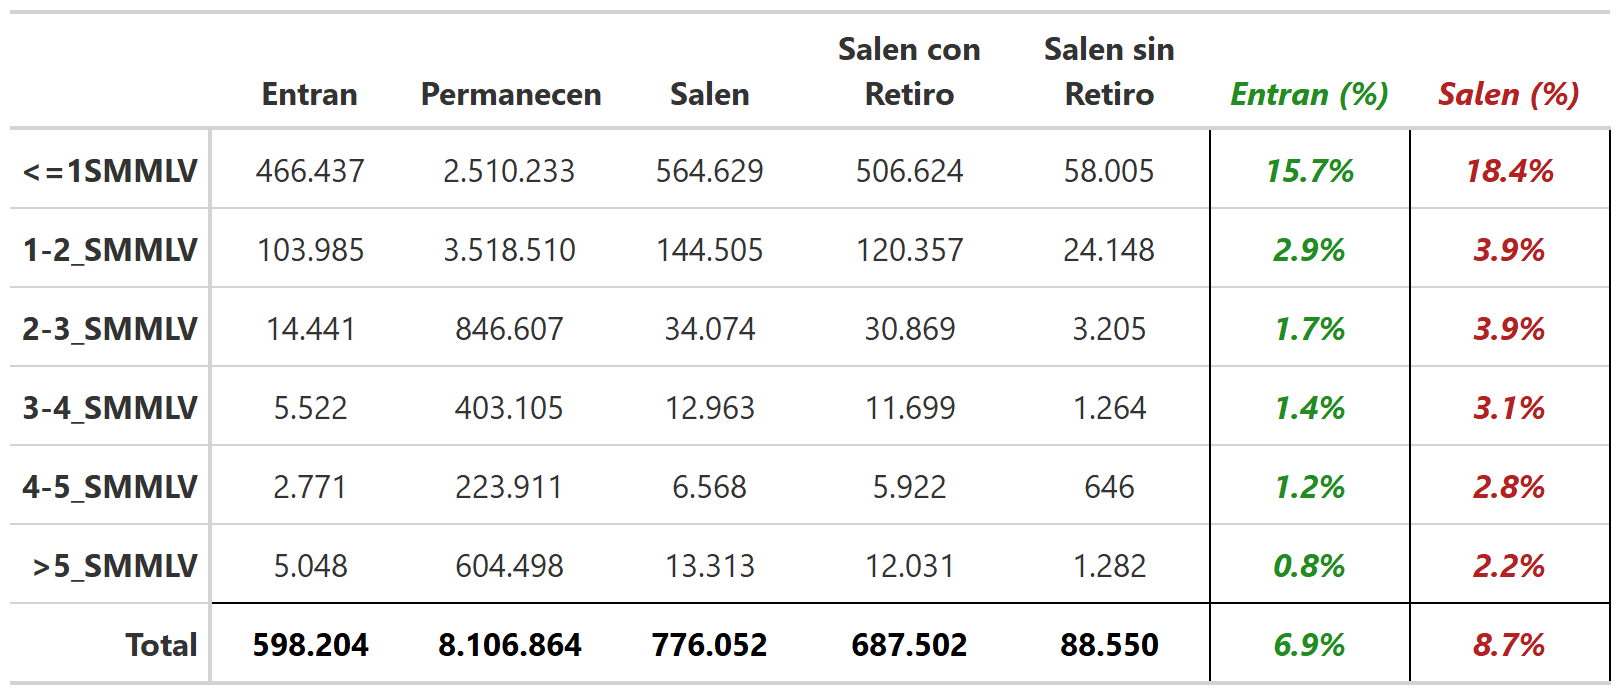
\includegraphics[width = 15cm]{results/02_longitudinal/salida_resumen_dependientes_interes_21.png}
\caption{Matriz dinámica pareada dependientes sector privado Noviembre - Diciembre 2021}%
\label{tabla:sector_privado:matriz_dinamica_mes_interes_21}
\end{table}

\begin{table}[!htbp]
\centering
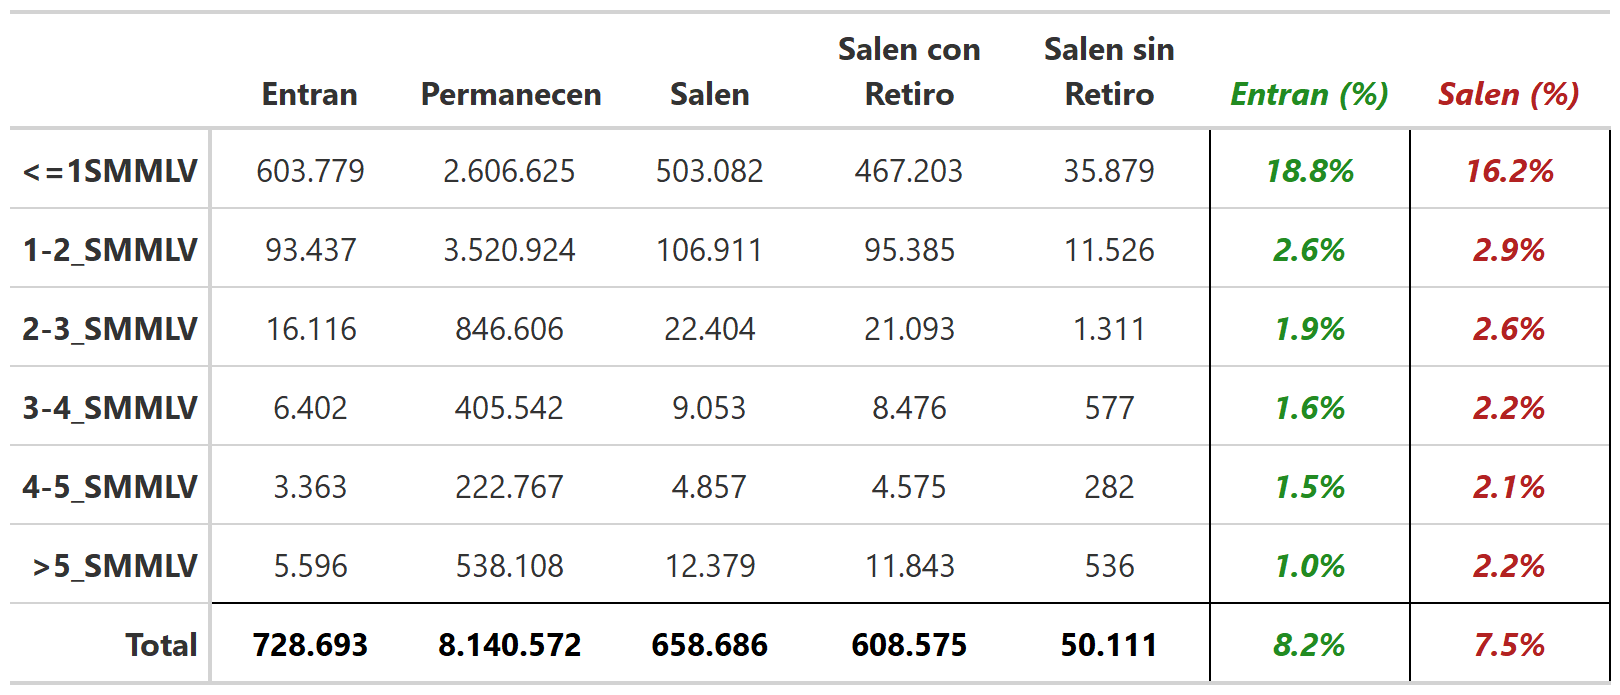
\includegraphics[width = 15cm]{results/02_longitudinal/salida_resumen_dependientes_referencia_21.png}
\caption{Matriz dinámica pareada dependientes sector privado Octubre - Noviembre 2021}%
\label{tabla:sector_privado:matriz_dinamica_mes_referencia_21}
\end{table}

%%%%%
\FloatBarrier
\paragraph{Relaciones laborales que permanecieron}\mbox{}\\

De los dependientes del sector privado que permanecieron en el SPS, se evidenció que los mayores cambios en el rango IBC entre Noviembre  y Diciembre se dan en 1 SMMLV. Por ejemplo, existe un 25.2\% de cotizantes que aumentaron de 4 y 5 SMMLV para Noviembre, a Más de 5 SMMLV para Diciembre de 2021. De igual manera la disminución del 11.6\% se da en el cambio entre 3 y 4 SMMLV. La categoría más estable en este caso corresponde a los cotizantes entre 1 y 2 SMMLV (86.5\%) que permanencen en el mismo rango para los dos meses. 

Al comparar la distribución porcentual de quienes disminuyen su IBC entre Noviembre y Diciembre, se pudo ver que en 2020 el porcentaje de cotizantes es ligeramente menor a lo ocurrido en 2021 (Ver Cuadro \ref{tabla:sector_privado:matriz_transicion_mes_interes_20}). Sin embargo, estos valores no superan lo ocurrido en 2019 (Ver Cuadro \ref{tabla:sector_privado:matriz_transicion_mes_interes_20}). En cuanto a los que incrementan su IBC, se observó que los cotizantes de menos de 2 SMMLV incrementaron relativamente sus montos de IBC. Generalmente este aumento no es de más de 1 SMMLV (14.8\%, 5.2\% para 2021). Por otro lado aquellos que cotizaron entre 3 y 5 SMMLV mostraron una disminución comparativa en cuanto al aumento en el IBC. Dicha variación ses más grande en los cotizantes entre 4 y 5 SMMLV (alrededor de 1\% comparado con 2020 y 2019). 

\begin{table}[!htbp]
\label{tabla:sector_privado:matriz_transicion_mes_interes_21}
\centering
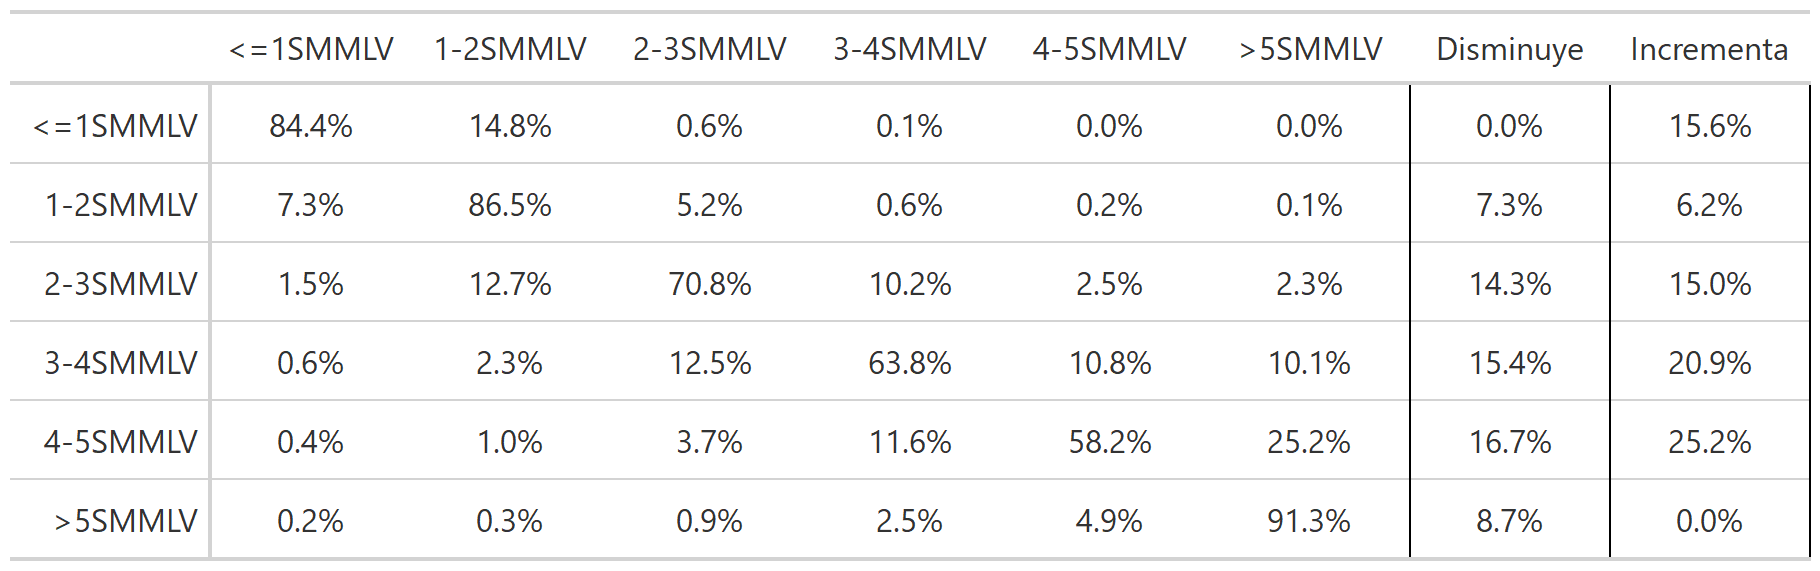
\includegraphics[width = 15cm]{results/02_longitudinal/salida_matriz_transicion_dependientes_21.png}
\caption{Matriz de transición sector privado Noviembre(filas) - Diciembre(columnas) 2021}%
\label{tabla:dependientes:matriz_transicion}
\end{table}

\FloatBarrier
\paragraph{Análisis por sección económica}\mbox{}\\

Se observó que para este mes los cambios en la distribución de actividades no son sustanciales. Existe una concentración de actividades económicas es los sectores de servicios administrativos (20.2\%), comercio (14.7\%) e industria manufacturera (11.8\%). De acuerdo al decrecimiento observado en el número de relaciones laborales entre Noviembre y Diciembre de 2021, el cambio se concentro en las actividades económicas de educación (-15.3\%) y Construcción (-5.8\%). En términos de variaciones anuales se evidenció que los sectores que crecieron en más de un 10\% fueron: \textbf{información y telecomunicaciones} creció en 20\%, \textbf{Alojamiento y servicio de comida} en 19.8\%, \textbf{Actividades de servicios administrativos y de apoyo} en 11\%. El sector de \textbf{Administración pública y defensa} creció negativamente en 1.3\%. 

\begin{table}[!htbp]
\label{tabla:sector_privado:actividad_economica_mes_interes_21}
\centering
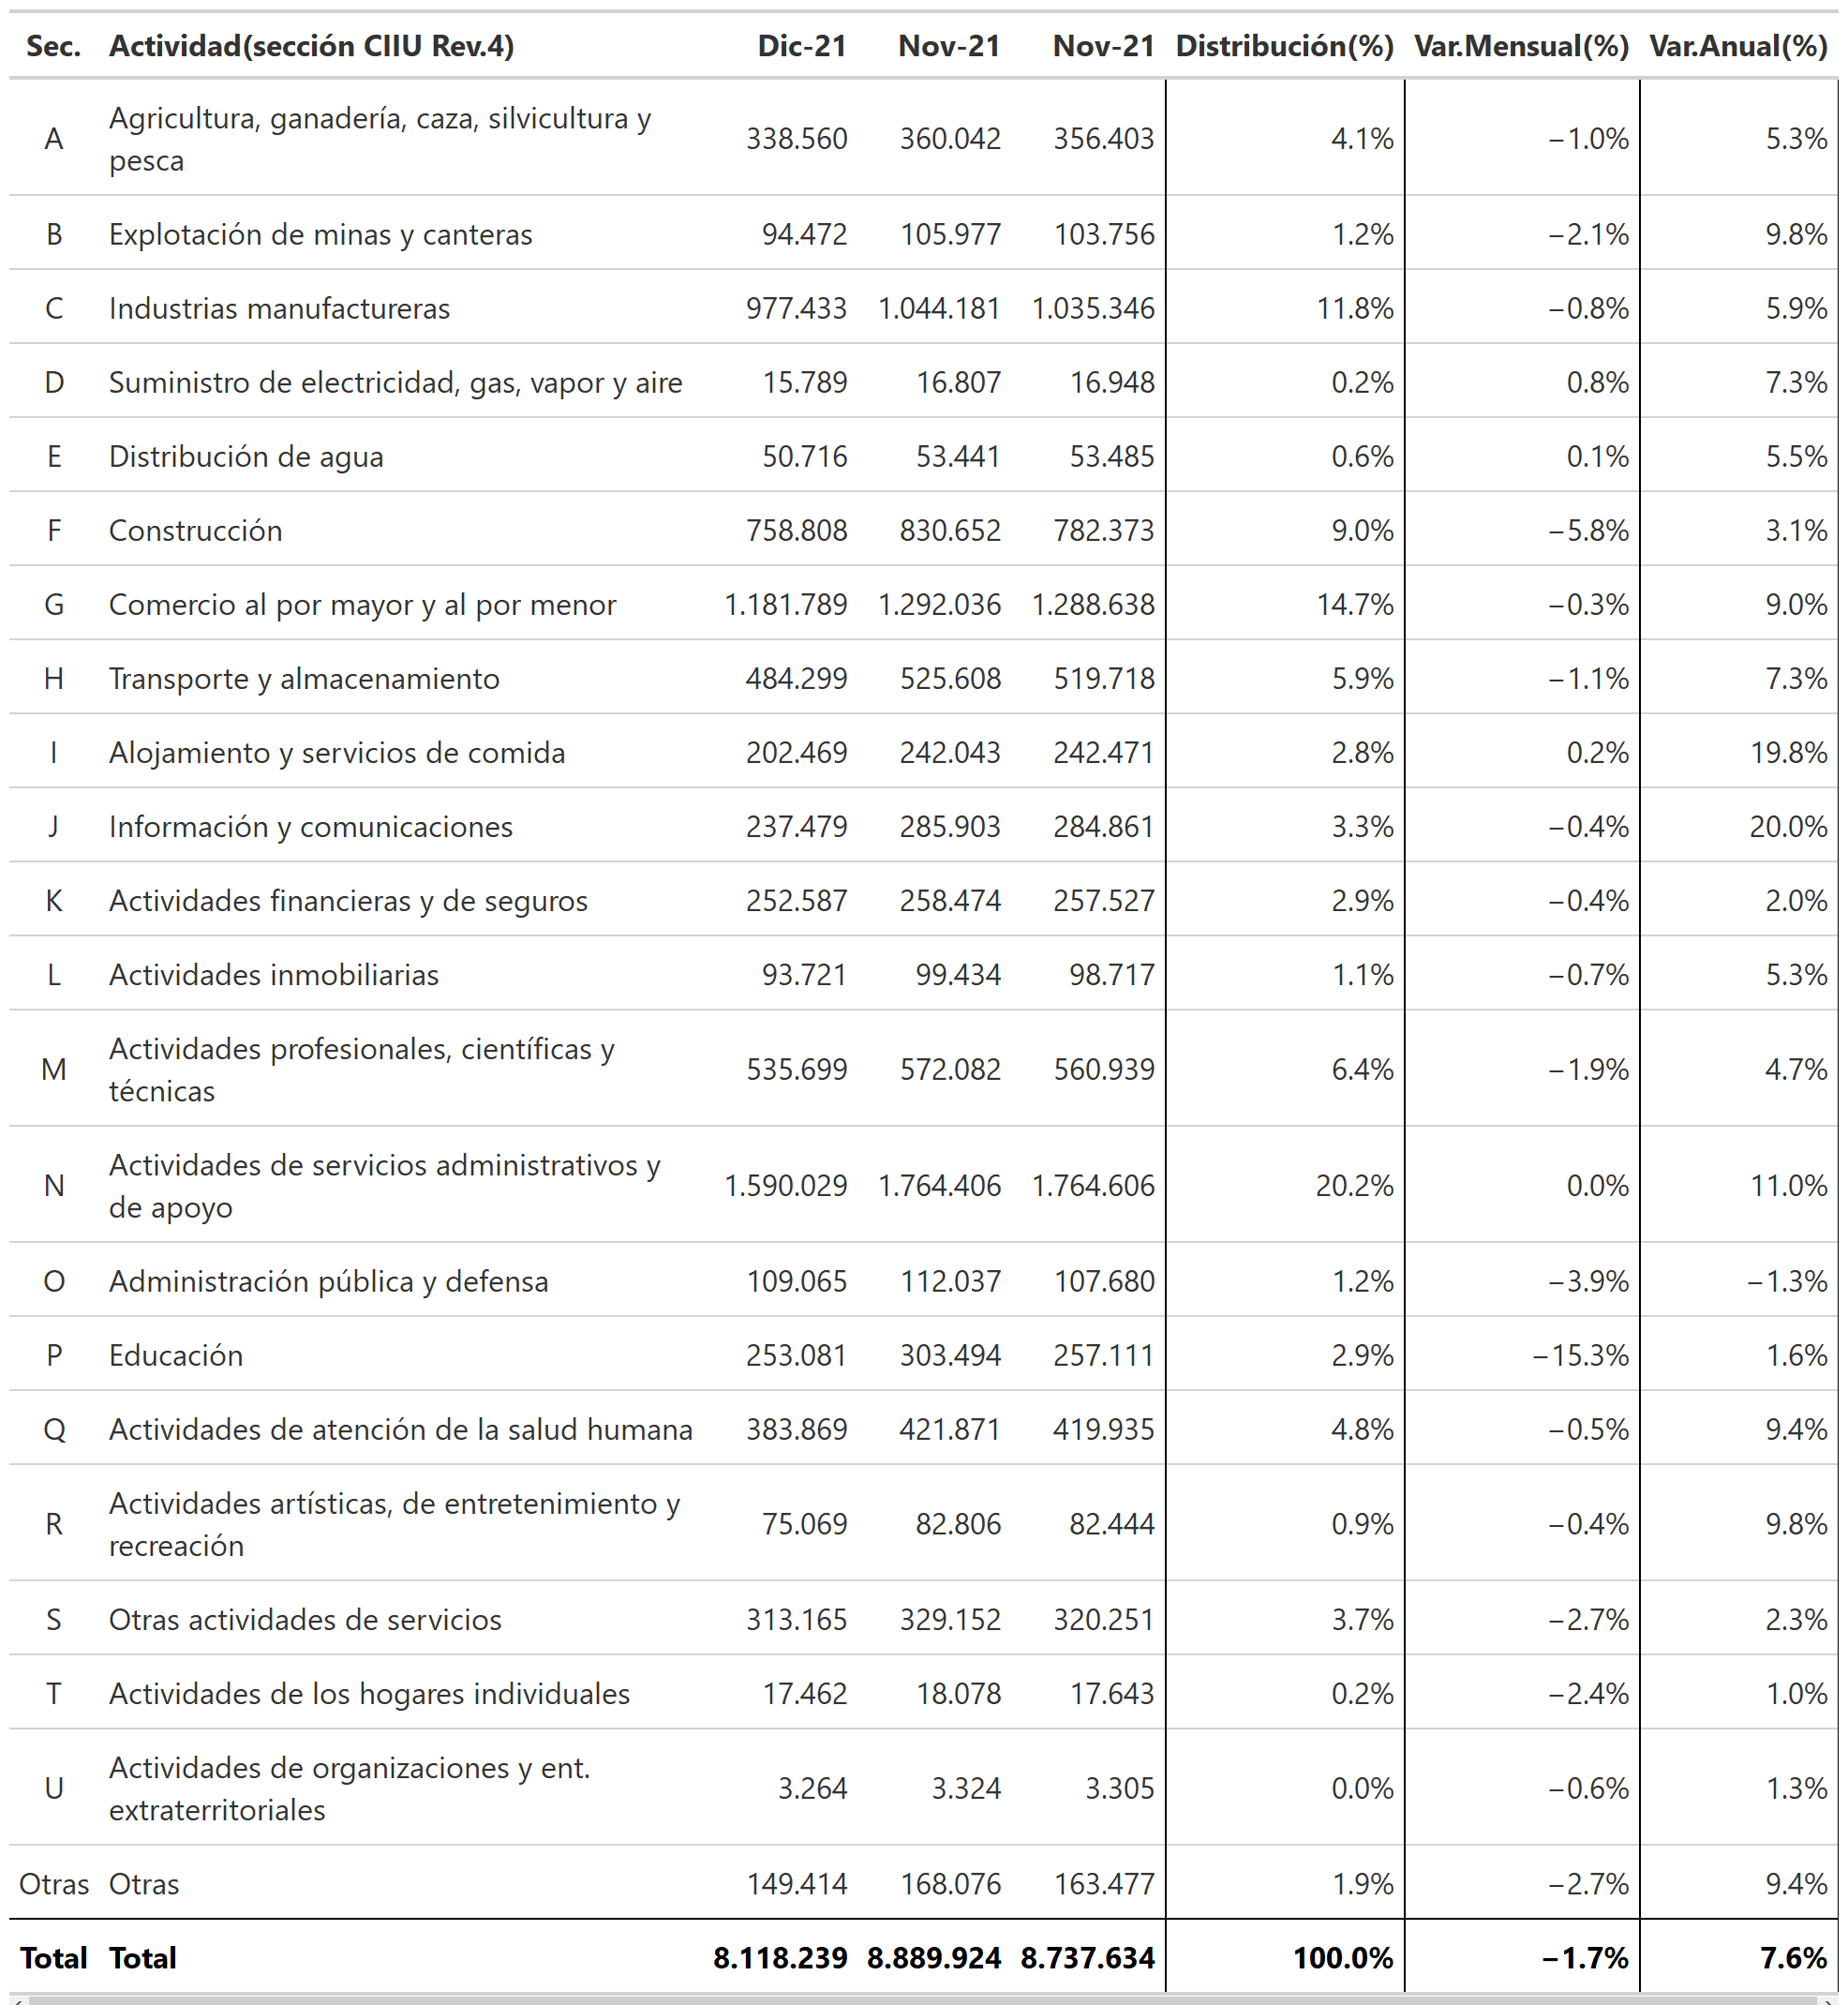
\includegraphics[width = 15cm]{results/02_longitudinal/salida_act_econ_dependientes_21.png}
\caption{Total cotizantes sector privado  por sección económica}%
\end{table}
%grfico 1 dinamicas del sector privado 

\subsection{Independientes}

El número de relaciones laborales que permanecen en el SPS es de \textbf{2.059.803}, lo cual representa un crecimiento negativo de -3.3\% de lo presentado en Noviembre de 2021. En cuanto al comparativo con las relaciones laborales que entran, se observó un crecimiento negativo de -11.2\%. Por otro lado las salidas aumentaron en un 51.2\%.  En términos de los cotizantes independientes se observó que aquella relaciones laborales por menos de 1 SMMLV en el IBC son las que presentan mayores variaciones. #l 6.3\% entraron  mientras que el 10.3\% salieron del SPS. Sin embargo, para aquellas entre 1 y 2 SMMLV el porcentaje de aquellas que salen (9.1\%) es considerablemente mayor a las que salen (3.8\%). Este comportamiento se mantiene a hasta aquellas con 5 SMMLV. Entre tanto para las mayores a 5 SMMLV el porcentaje de las que entran es 1.1\% mayor a las que salen. 

Se identificó que relaciones laborales en Diciembre 2021 por más de 3 SMMLV tienen alrededor de 2\% más de salidas que lo presentado en Diciembre 2019 y 2020. Es importante resaltar que el número de las nuevas relaciones al igual que las salidas del SPS en Diciembre 2021 es mayor que lo presentado en años anteriores . Véase los Cuadros \ref{tabla:independientes:matriz_dinamica_mes_interes_19} y \ref{tabla:independientes:matriz_dinamica_mes_interes_20} para ver más otros detalles del comparativo.

\subsubsection{Dinámica de entradas y salidas del SPS}
\begin{table}[!htbp]
\label{tabla:independientes:matriz_dinamica_mes_interes_21}
\centering
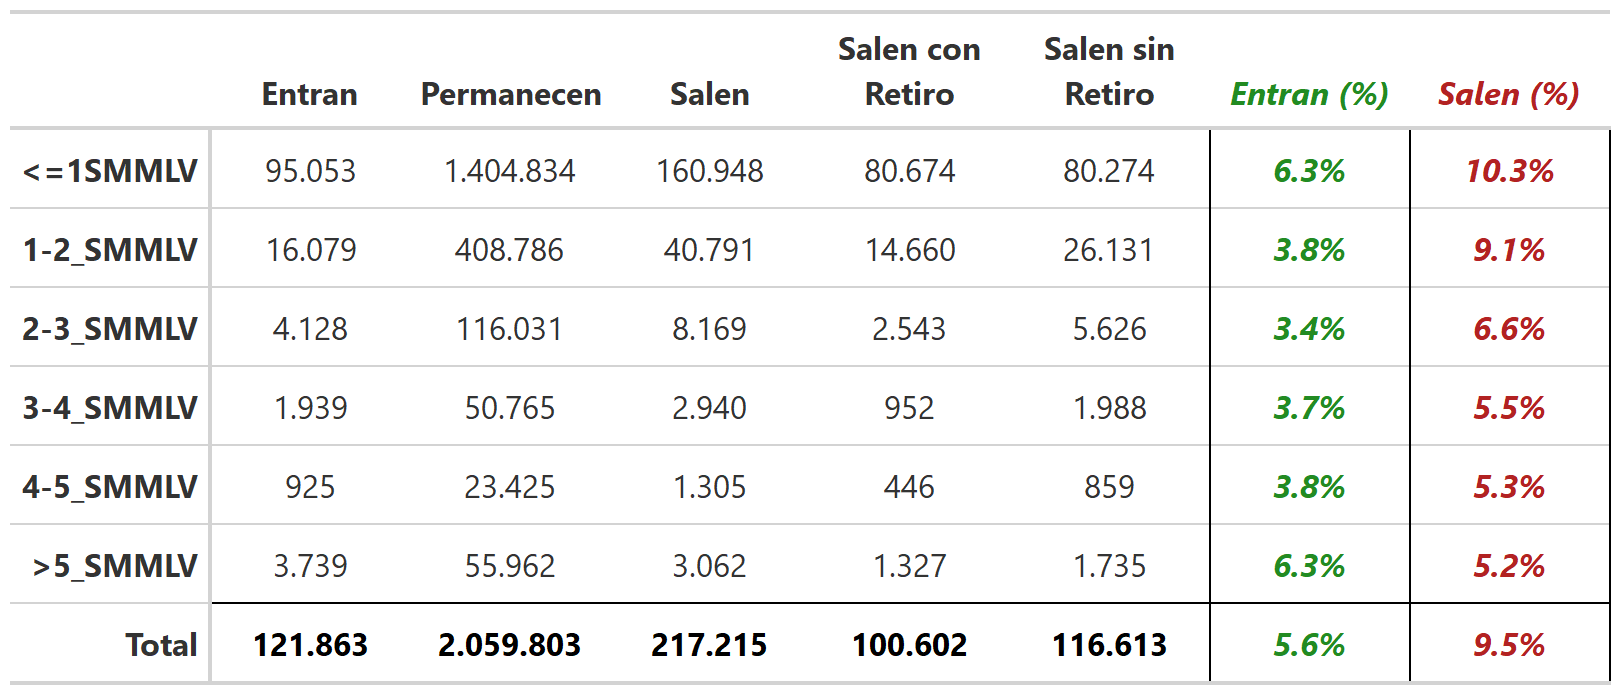
\includegraphics[width = 15cm]{results/02_longitudinal/salida_resumen_independientes_interes_21.png}
\caption{Matriz dinámica pareada independientes Noviembre - Diciembre 2021}%
\end{table}

\begin{table}[!htbp]
\label{tabla:independientes:matriz_dinamica_mes_referencia_21}
\centering
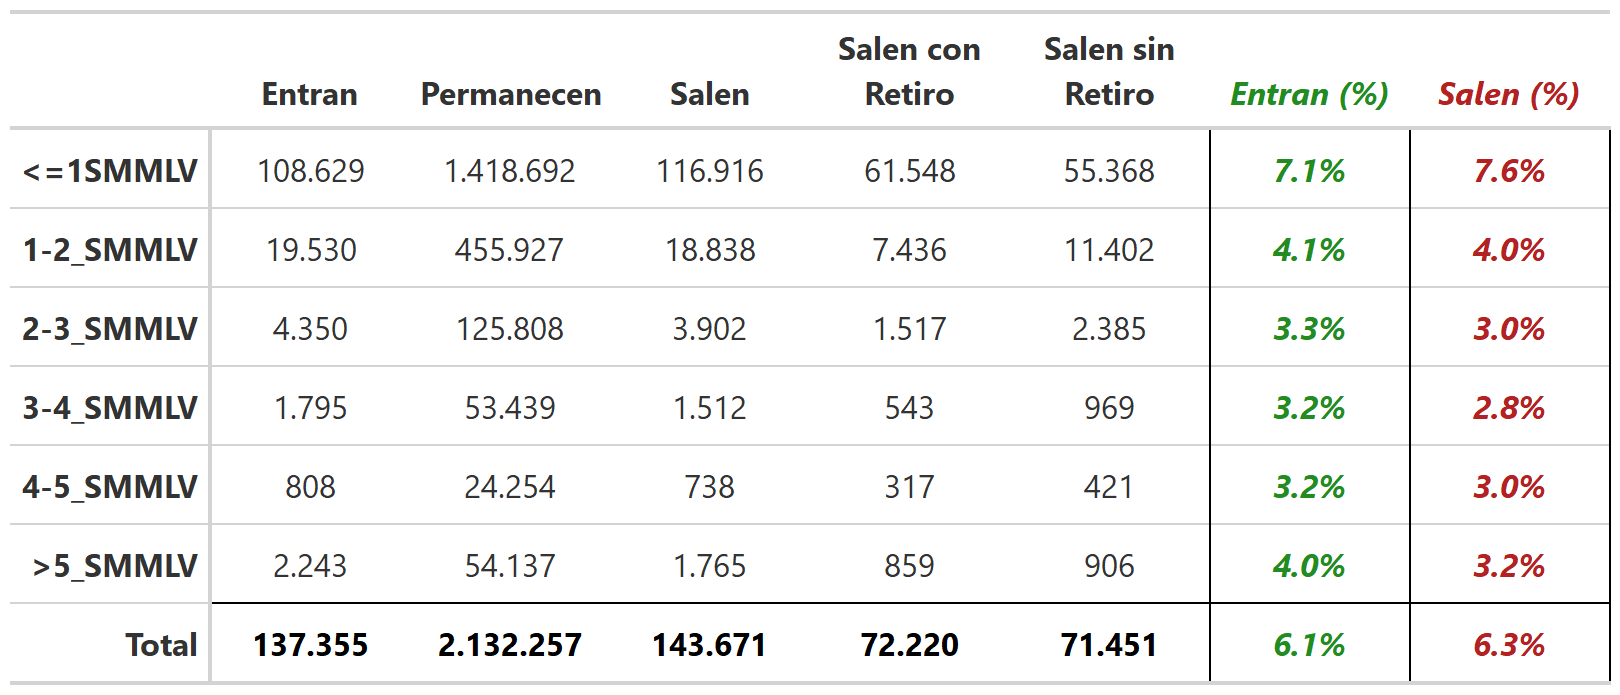
\includegraphics[width = 15cm]{results/02_longitudinal/salida_resumen_independientes_referencia_21.png}
\caption{Matriz dinámica pareada independientes Octubre - Noviembre 2021}%
\end{table}


\FloatBarrier
\paragraph{Relaciones laborales que permanecieron}\mbox{}\\


Las relaciones laborales que permanecieron 

\begin{table}[!htbp]
\centering
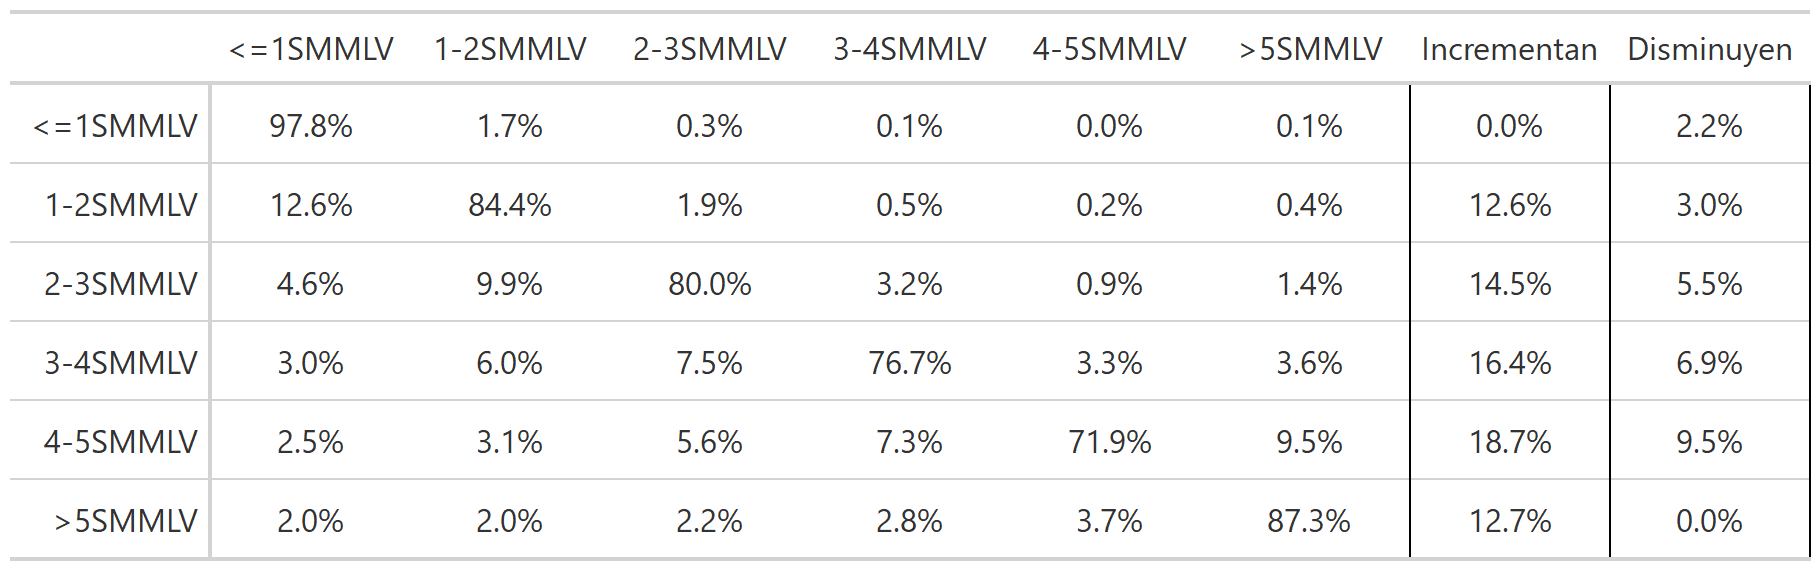
\includegraphics[width = 18cm]{results/02_longitudinal/salida_matriz_transicion_independientes_21.png}
\caption{Matriz de transición independientes Noviembre - Diciembre 2021}%
\label{tabla:independientes:matriz_transicion_mes_interes_21}
\end{table}

\FloatBarrier
\paragraph{Análisis por sección económica}\mbox{}\\

\begin{table}[!htbp]
\centering
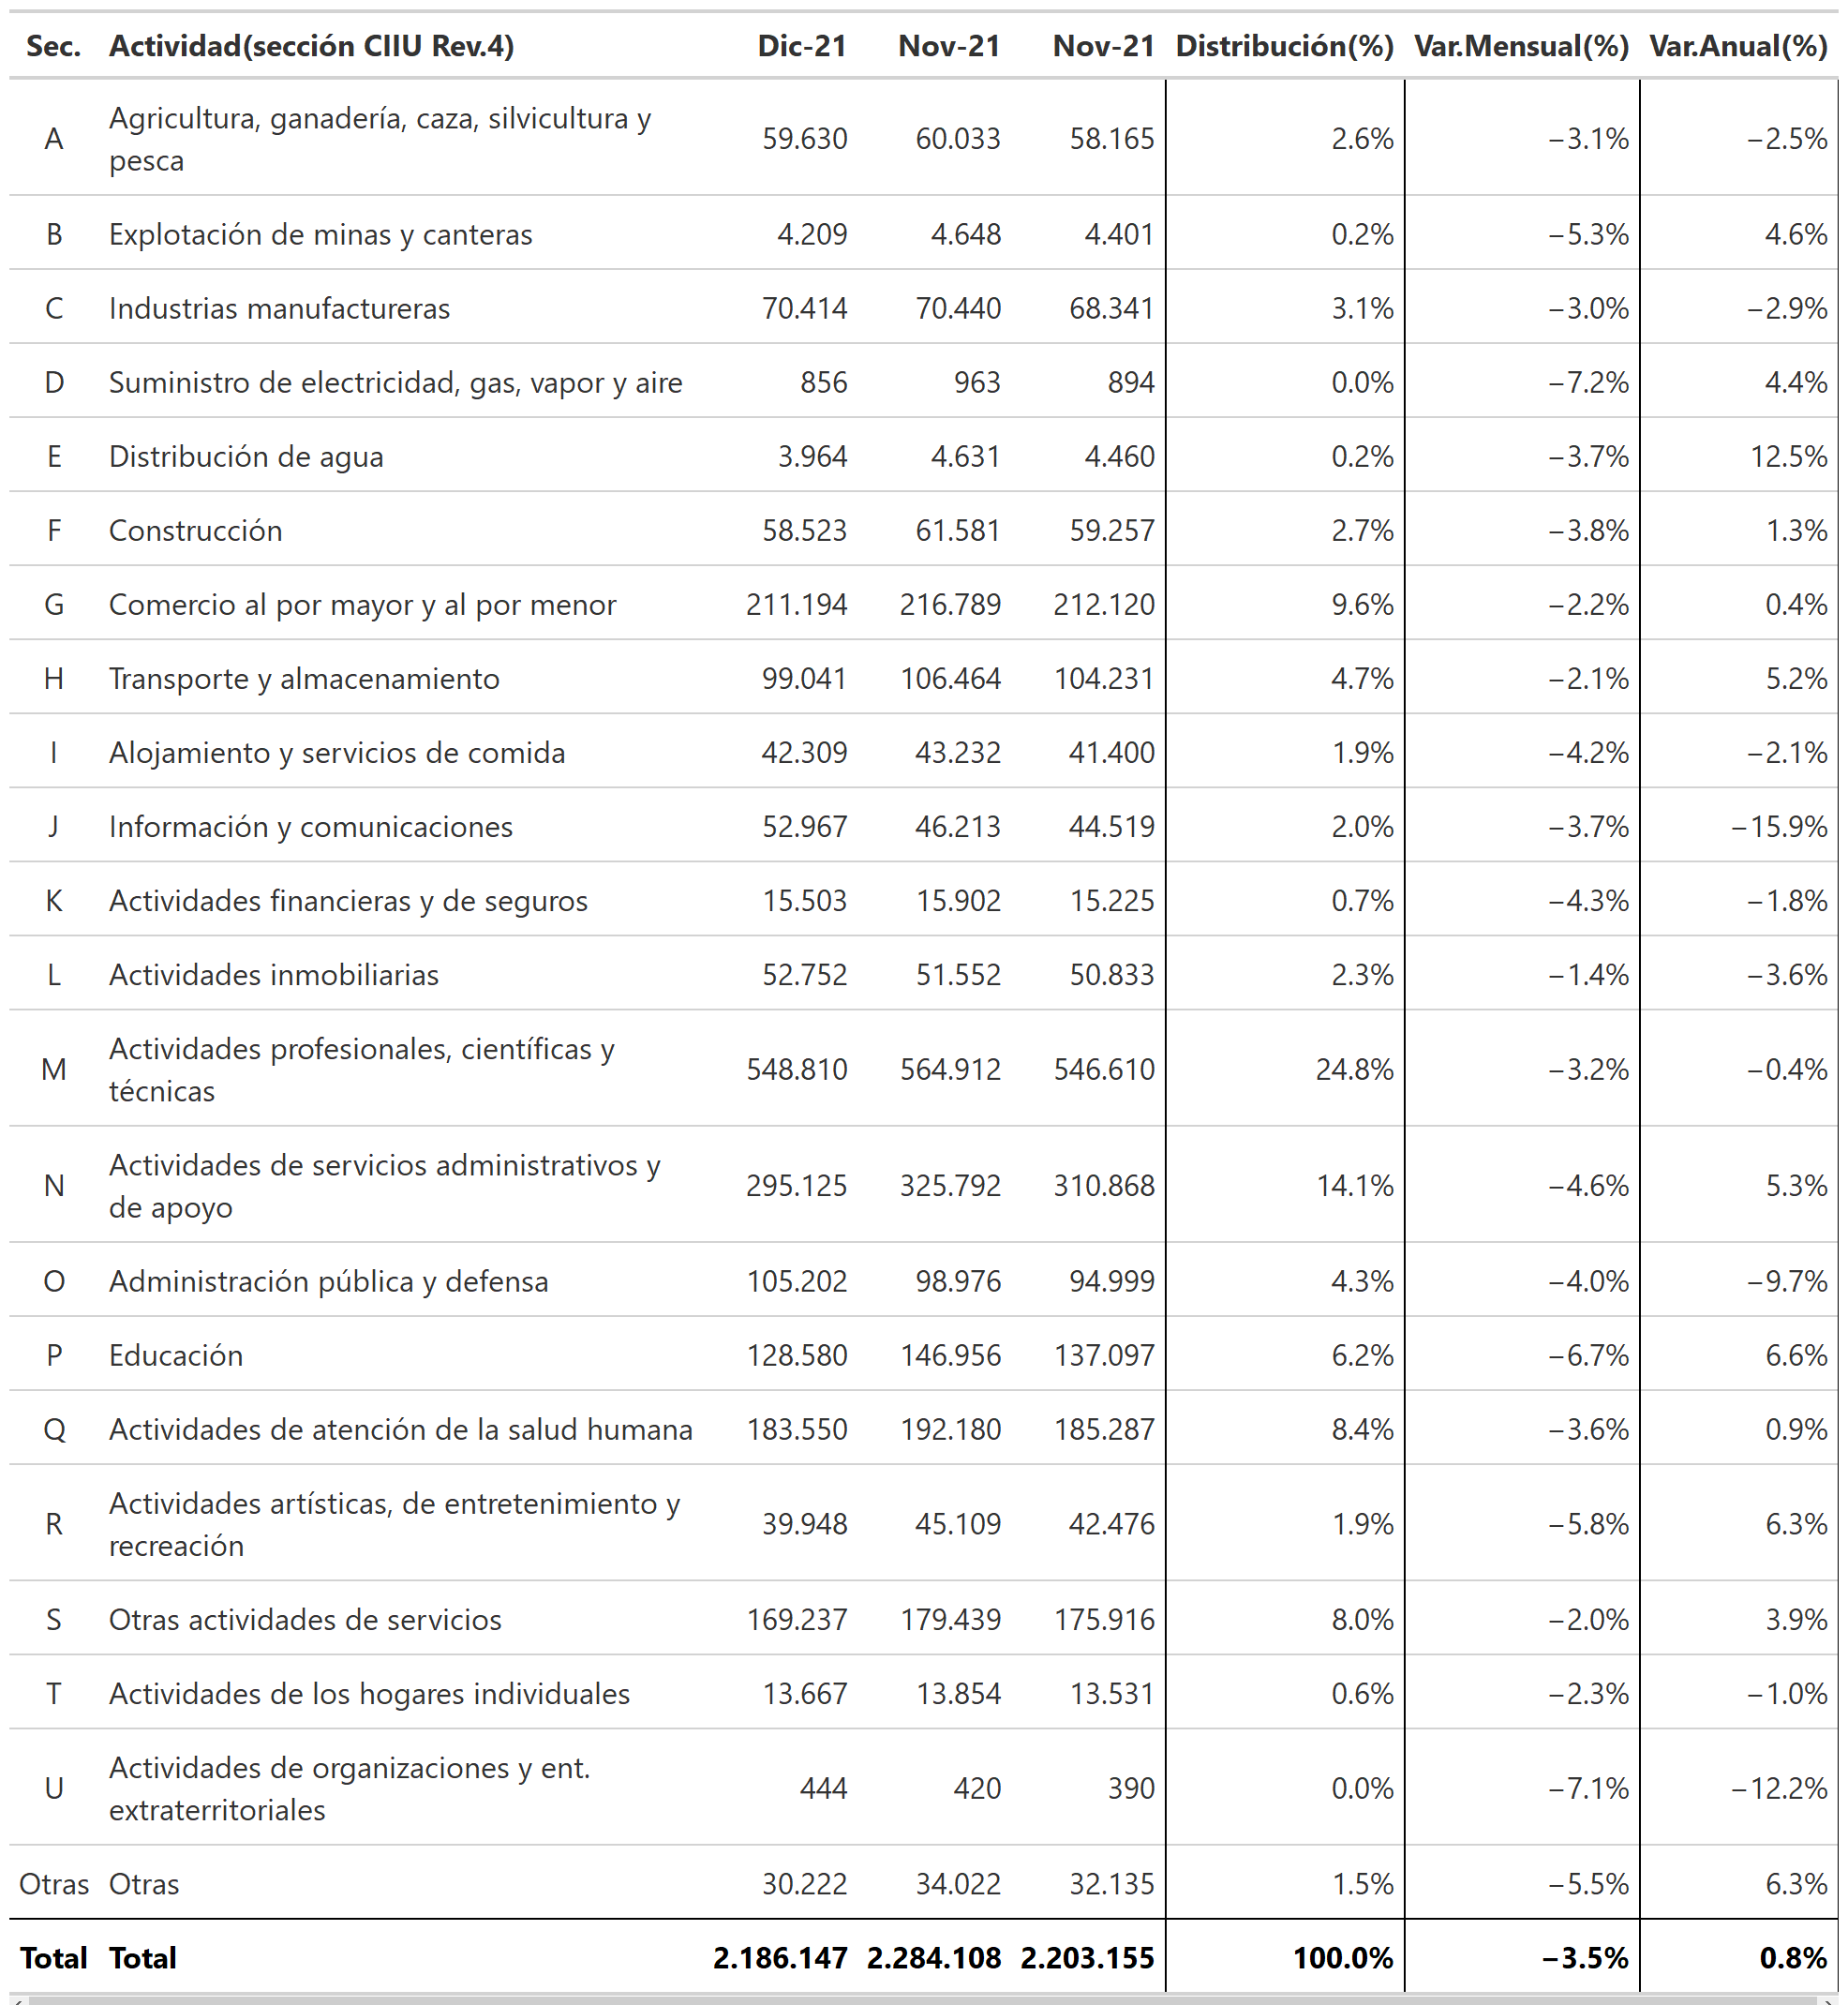
\includegraphics[width = 15cm]{results/02_longitudinal/salida_act_econ_independientes_21.png}
\caption{Total cotizantes independientes por sección económica}%
\label{tabla:independientes:actividad_economica_mes_interes_21}
\end{table}

\FloatBarrier
\subsection{Análisis demográfico dependientes sector privado e independientes}

\begin{figure}[!htbp]
\centering
\begin{minipage}{0.5\textwidth}
  \centering
  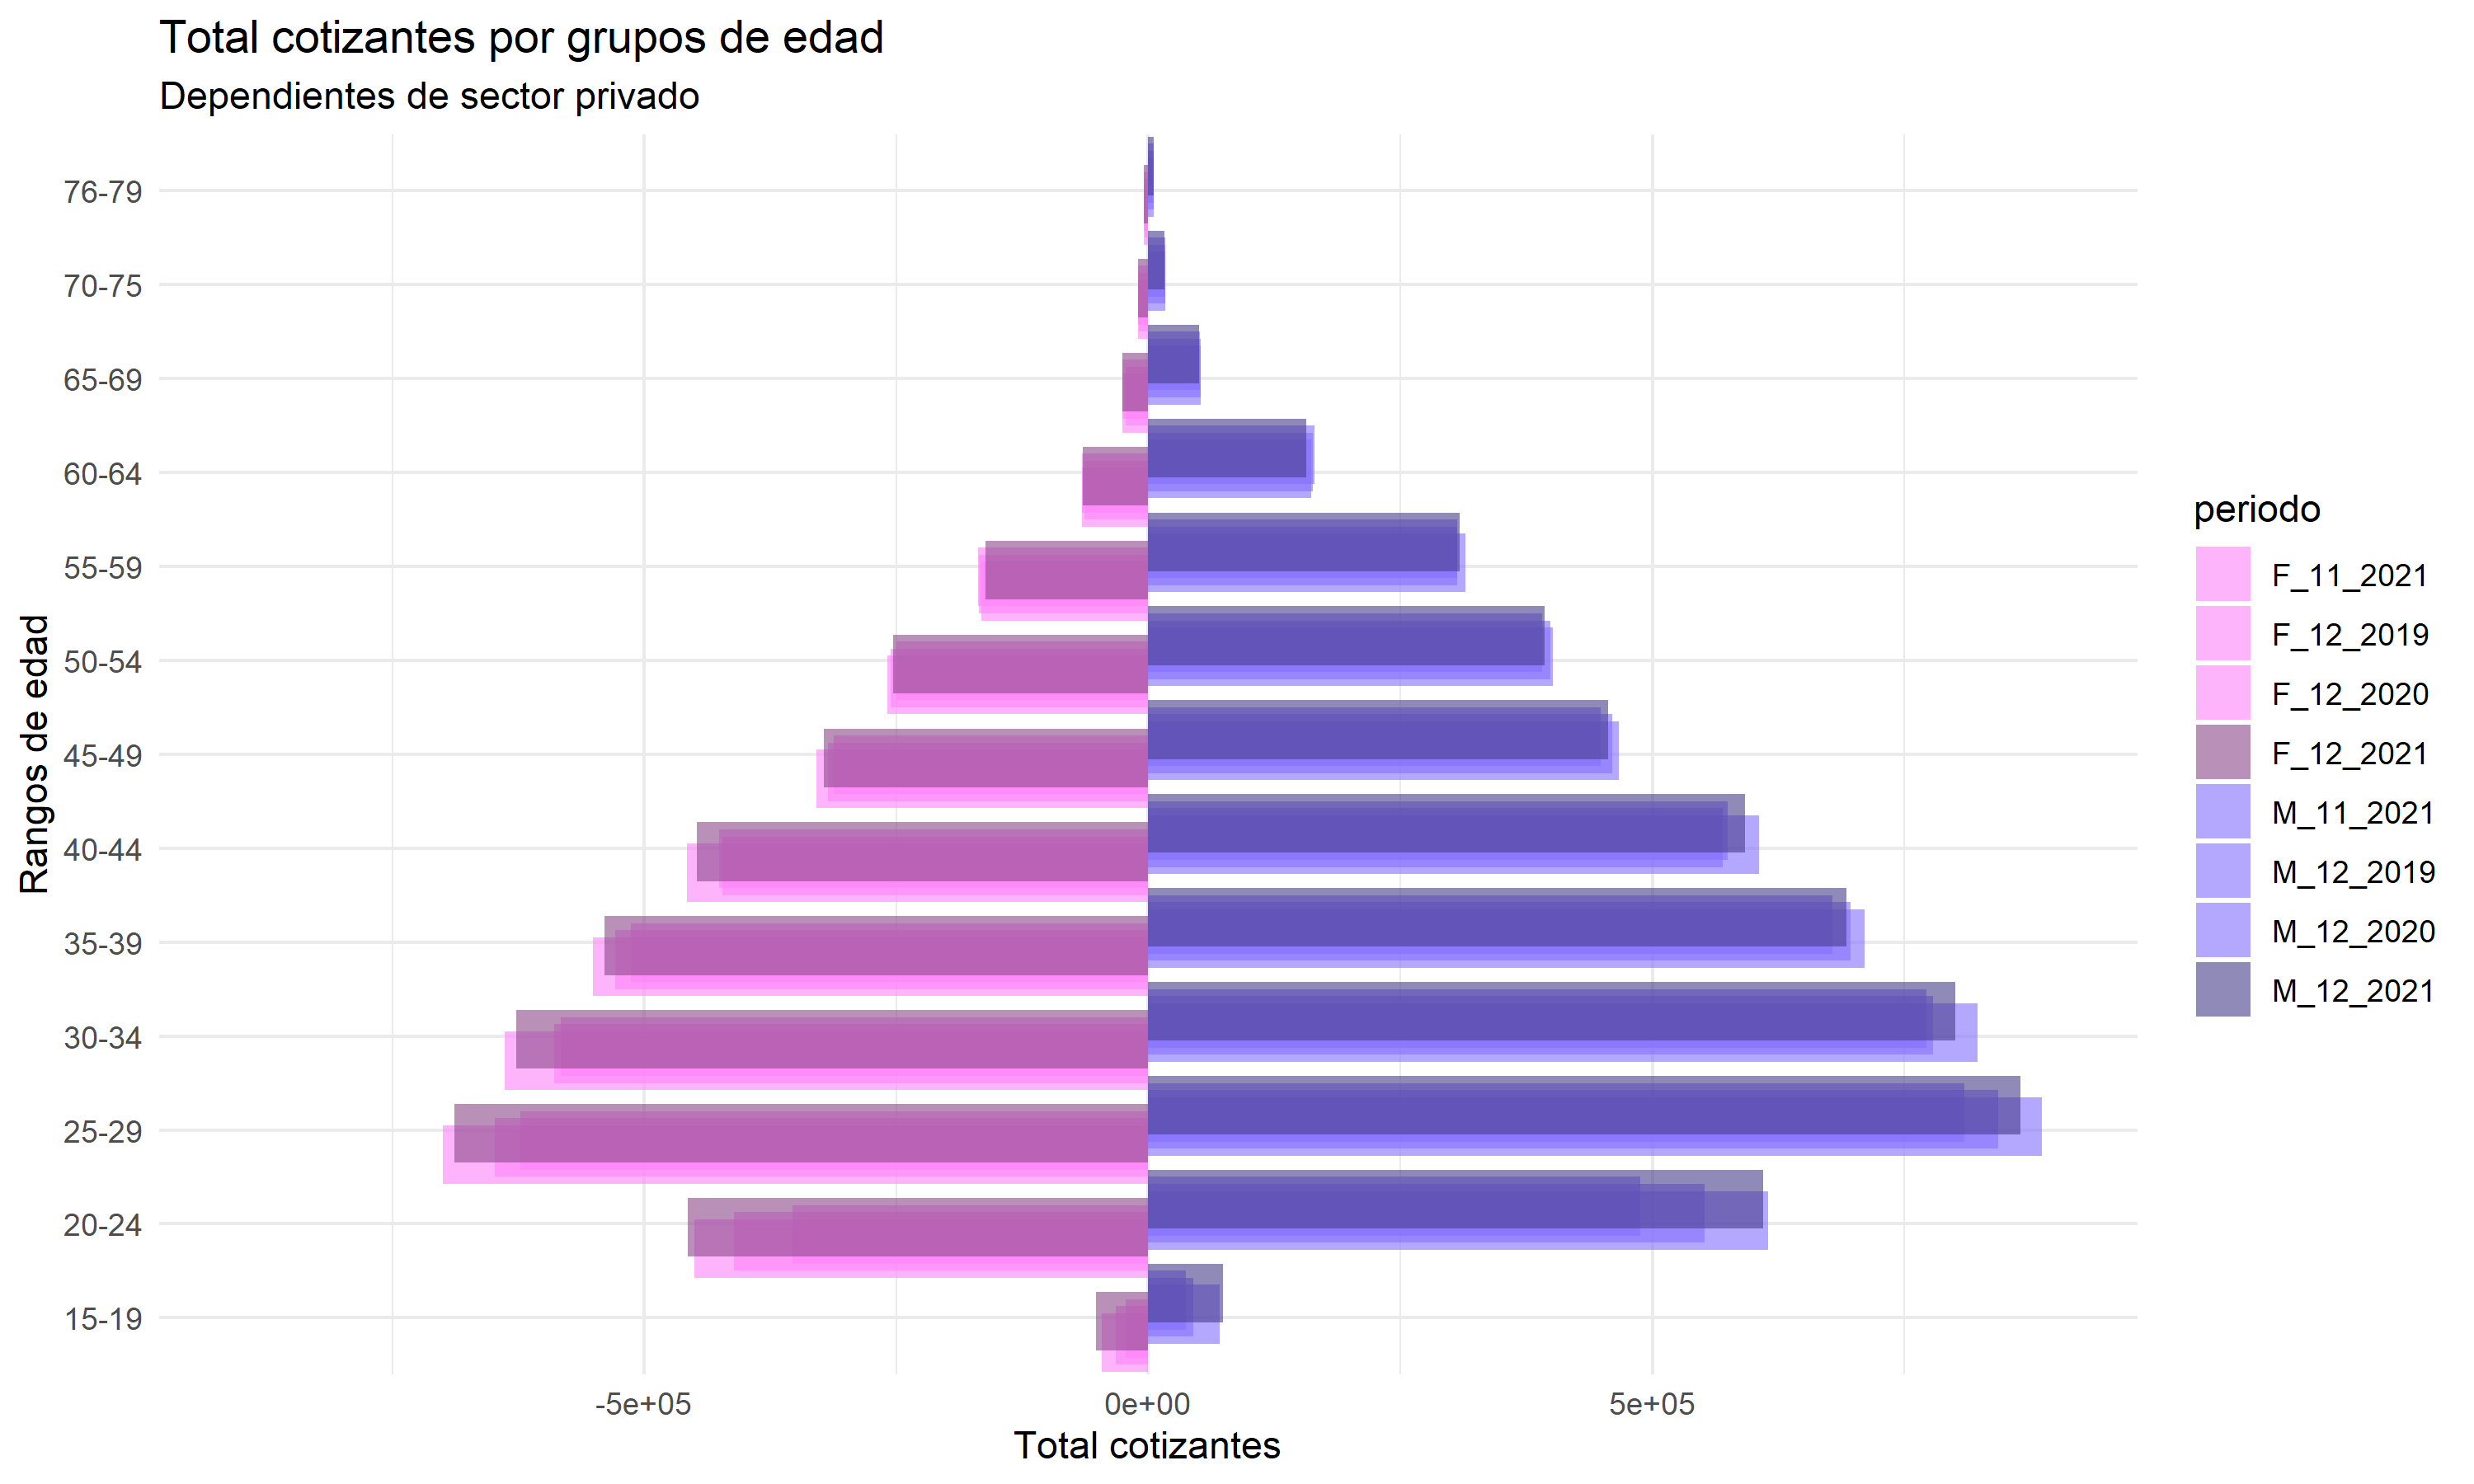
\includegraphics[width=\linewidth]{figures/02_longitudinal/salidas_piramide_dependientes.png}
\end{minipage}%
\begin{minipage}{0.5\textwidth}
  \centering
  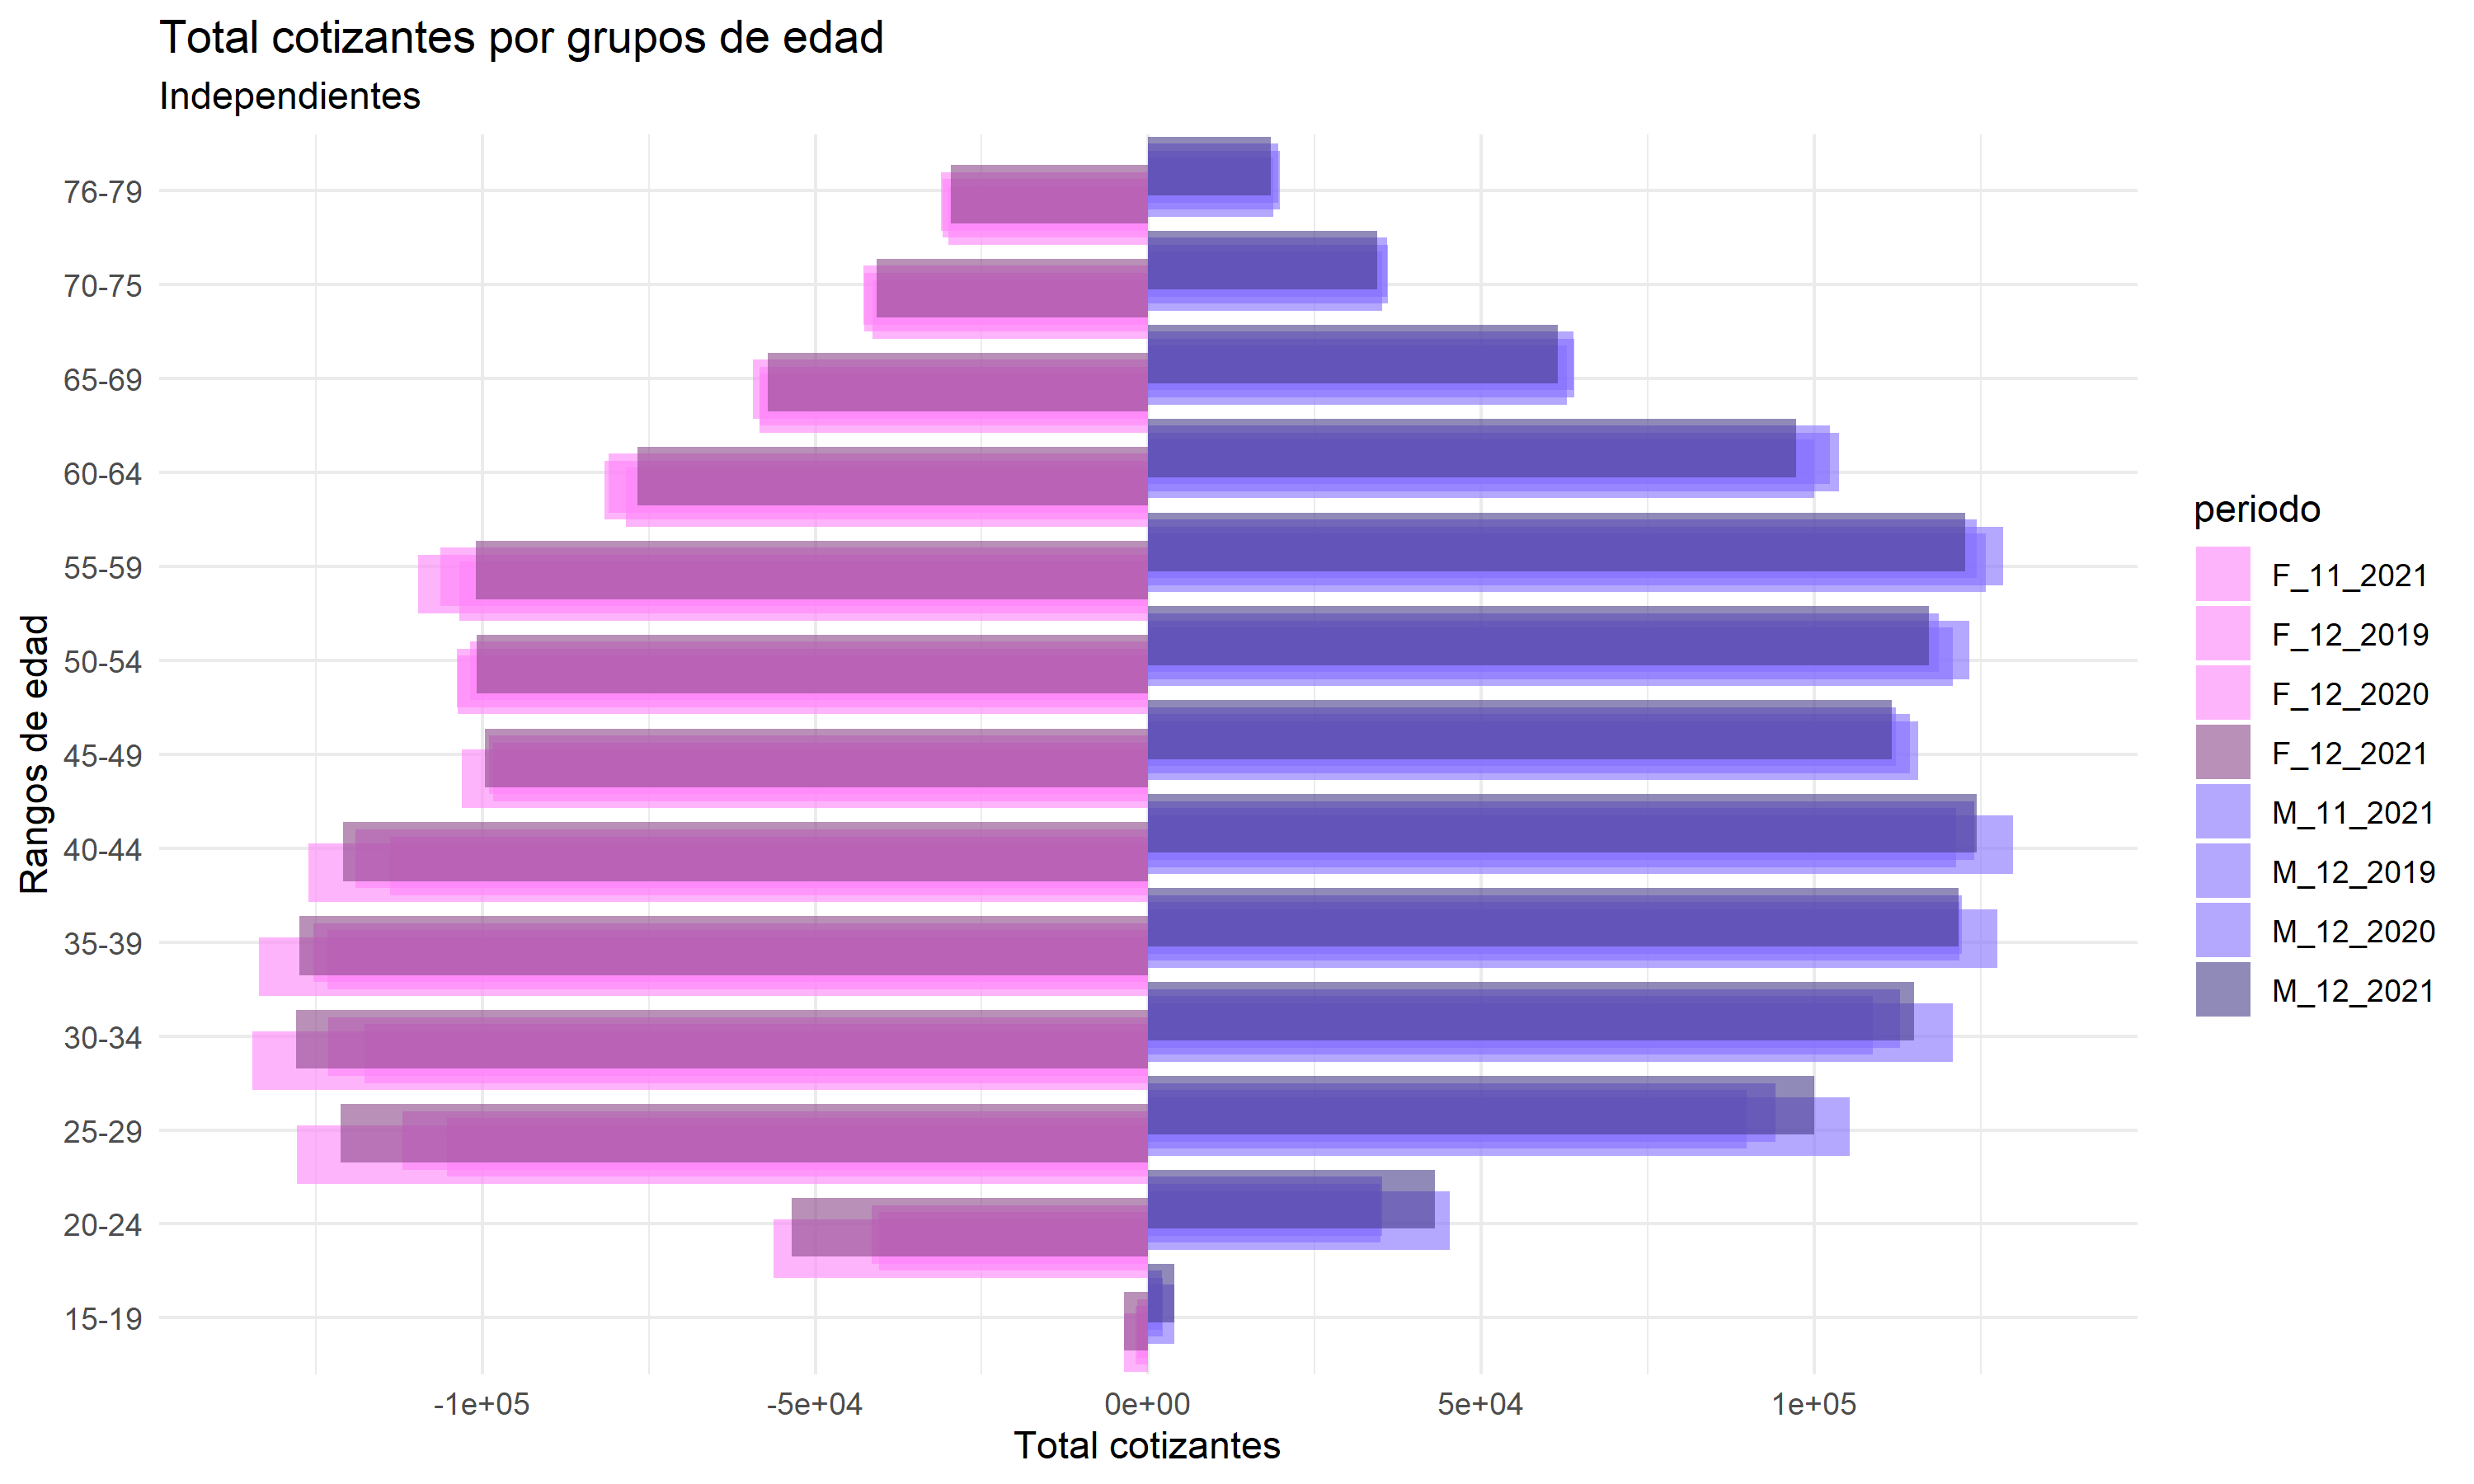
\includegraphics[width=\linewidth]{figures/02_longitudinal/salidas_piramide_independientes.png}
\end{minipage}
\caption{Porcentaje de entradas (izq.) y salidas (der.) por año}
\label{figura:piramides}
\end{figure}


